\documentclass{amsart}
\usepackage[margin=1.5in]{geometry} 
\usepackage{amsmath}
\usepackage{tcolorbox}
\usepackage{amssymb}
\usepackage{amsthm}
\usepackage{lastpage}
\usepackage{fancyhdr}
\usepackage{accents}
\usepackage{hyperref}
\usepackage{xcolor}
\usepackage{color}
\usepackage{euscript}
\usepackage[bbgreekl]{mathbbol}
\DeclareSymbolFontAlphabet{\mathbb}{AMSb} % to ensure \mathbb does not change
\DeclareSymbolFontAlphabet{\mathbbl}{bbold}
% Fields
\newcommand{\CC}{\mathbb{C}}
\newcommand{\RR}{\mathbb{R}}
\newcommand{\QQ}{\mathbb{Q}}
\newcommand{\ZZ}{\mathbb{Z}}
\newcommand{\NN}{\mathbb{N}}

% mathcal letters
\newcommand{\Acal}{\mathcal{A}}
\newcommand{\Bcal}{\mathcal{B}}
\newcommand{\Ccal}{\mathcal{C}}
\newcommand{\Dcal}{\mathcal{D}}
\newcommand{\Ecal}{\mathcal{E}}
\newcommand{\Fcal}{\mathcal{F}}
\newcommand{\Gcal}{\mathcal{G}}
\newcommand{\Hcal}{\mathcal{H}}
\newcommand{\Ical}{\mathcal{I}}
\newcommand{\Jcal}{\mathcal{J}}
\newcommand{\Kcal}{\mathcal{K}}
\newcommand{\Lcal}{\mathcal{L}}
\newcommand{\Mcal}{\mathcal{M}}
\newcommand{\Ncal}{\mathcal{N}}
\newcommand{\Ocal}{\mathcal{O}}
\newcommand{\Pcal}{\mathcal{P}}
\newcommand{\Qcal}{\mathcal{Q}}
\newcommand{\Rcal}{\mathcal{R}}
\newcommand{\Scal}{\mathcal{S}}
\newcommand{\Tcal}{\mathcal{T}}
\newcommand{\Ucal}{\mathcal{U}}
\newcommand{\Vcal}{\mathcal{V}}
\newcommand{\Wcal}{\mathcal{W}}
\newcommand{\Xcal}{\mathcal{X}}
\newcommand{\Ycal}{\mathcal{Y}}
\newcommand{\Zcal}{\mathcal{Z}}

% abstract categories
\newcommand{\Asf}{\mathsf{A}}
\newcommand{\Bsf}{\mathsf{B}}
\newcommand{\Csf}{\mathsf{C}}
\newcommand{\Dsf}{\mathsf{D}}
\newcommand{\hsf}{\mathsf{h}}
\newcommand{\Rsf}{\mathsf{R}}
\newcommand{\Ssf}{\mathsf{S}}
\newcommand{\Tsf}{\mathsf{T}}
\newcommand{\Lsf}{\mathsf{L}}
\newcommand{\ksf}{\mathsf{k}}
\newcommand{\ysf}{\mathsf{y}}

% infinity categories
\newcommand{\Ascr}{\EuScript{A}}
\newcommand{\Bscr}{\EuScript{B}}
\newcommand{\Cscr}{\EuScript{C}}
\newcommand{\Dscr}{\EuScript{D}}
\newcommand{\Escr}{\EuScript{E}}
\newcommand{\catPr}{\mathsf{Pr}}

% algebraic geometry
\newcommand{\spec}{\operatorname{Spec}}
\newcommand{\proj}{\operatorname{Proj}}

% categories 
\newcommand{\id}{\mathrm{id}}
\newcommand{\Obj}{\mathrm{Obj}}
\newcommand{\Mor}{\mathrm{Mor}}
\newcommand{\Hom}{\mathrm{Hom}}
\newcommand{\Aut}{\mathrm{Aut}}
\newcommand{\Sets}{\mathsf{Sets}}
\newcommand{\SSets}{\mathsf{SSets}}
\newcommand{\kVec}{\mathsf{Vec}_{k}}
\newcommand{\Alg}{\mathsf{Alg}}
\newcommand{\Ring}{\mathsf{Ring}}
\newcommand{\Mod}{\mathsf{Mod}}
\newcommand{\Grp}{\mathsf{Grp}}
\newcommand{\AbGrp}{\mathsf{AbGrp}}
\newcommand{\PSh}{\mathsf{PSh}}
\newcommand{\Sh}{\mathsf{Sh}}
\newcommand{\PSch}{\mathsf{PSch}}
\newcommand{\Sch}{\mathsf{Sch}}
\newcommand{\Top}{\mathsf{Top}}
\newcommand{\Com}{\mathsf{Com}}
\newcommand{\Coh}{\mathsf{Coh}}
\newcommand{\QCoh}{\mathsf{QCoh}}
\newcommand{\Opens}{\mathsf{Opens}}
\newcommand{\Opp}{\mathsf{Opp}}
\newcommand{\Cat}{\mathsf{Cat}}
\newcommand{\colim}{\operatorname{colim}}
\newcommand{\Grpd}{\mathsf{Grpd}}
\newcommand{\Fun}{\mathrm{Fun}}
\newcommand{\cofib}{\mathrm{cofib}}


% simplicial sets
\newcommand{\DDelta}{\Updelta}
\newcommand{\Sing}{\operatorname{Sing}}

% condensed math
\newcommand{\LCA}{\mathsf{LCA}}
\newcommand{\Cond}{\mathsf{Cond}}
\newcommand{\dom}{\operatorname{dom}}
\newcommand{\Cov}{\operatorname{Cov}}
\newcommand{\proet}{\mathsf{pro}\mathsf{\acute{e}}\mathsf{t}}
\newcommand{\et}{\mathsf{\acute{e}t}}
\newcommand{\Ab}{\mathsf{Ab}}
\newcommand{\ProFin}{\mathsf{ProFin}}
\newcommand{\ExtDiscHaus}{\mathsf{ExtDiscHaus}}
\newcommand{\CHaus}{\mathsf{CHaus}}

% K-theory
\newcommand{\Perf}{\mathsf{Perf}}
\newcommand{\MotLoc}{\mathsf{MotLoc}}
\newcommand{\St}{\mathsf{St}}
\newcommand{\Ex}{\mathsf{Ex}}
\newcommand{\Calk}{\mathsf{Calk}}
\newcommand{\Ind}{\mathsf{Ind}}
\newcommand{\Sp}{\mathsf{Sp}}
\newcommand{\Loc}{\mathsf{Loc}}
\newcommand{\ev}{\mathrm{ev}}
\newcommand{\coev}{\mathrm{coev}}
\newcommand{\dual}{\mathsf{dual}}
\setlength{\headheight}{40pt}


\newenvironment{solution}
  {\renewcommand\qedsymbol{$\blacksquare$}
  \begin{proof}[Solution]}
  {\end{proof}}
\renewcommand\qedsymbol{$\blacksquare$}

\usepackage{amsmath, amssymb, tikz, amsthm, csquotes, multicol, footnote, tablefootnote, biblatex, wrapfig, float, quiver, mathrsfs, cleveref, enumitem, upgreek, todonotes}
\addbibresource{refs.bib}
\theoremstyle{definition}
\newtheorem{theorem}{Theorem}[section]
\newtheorem{lemma}[theorem]{Lemma}
\newtheorem{corollary}[theorem]{Corollary}
\newtheorem{exercise}[theorem]{Exercise}
\newtheorem{question}[theorem]{Question}
\newtheorem{example}[theorem]{Example}
\newtheorem{proposition}[theorem]{Proposition}
\newtheorem{conjecture}[theorem]{Conjecture}
\newtheorem{remark}[theorem]{Remark}
\newtheorem{definition}[theorem]{Definition}
\numberwithin{equation}{section}
\setcounter{tocdepth}{1}

\setuptodonotes{color=blue!20, size=tiny}


\begin{document}
\large
\title[A Prismatic Primer]{A Primer on Prismatic Cohomology}
\author{Wern Juin Gabriel Ong}
\address{Universit\"{a}t Bonn, Bonn, D-53111}
\email{wgabrielong@uni-bonn.de}
\urladdr{https://wgabrielong.github.io/}
\maketitle
\section*{Preliminaries}
This document seeks to give a primer on the theory of prismatic cohomology first developed in Bhatt-Scholze's seminal article \cite{BSPrismatic} based primarily on the lecture course of G. Bosco at the Universit\"{a}t Bonn in the Summer 2024 semester \cite{Bosco} and of J. Ansch\"{u}tz at the Recent Advances in Algebraic K-Theory conference at the I'HES in Summer 2023 \cite{Anschutz}. In particular, no claims to completeness of proofs -- if at all given -- are made. 
\tableofcontents
\newpage
\section{Motivations}\label{sec: motivations}
Let $X$ be a scheme smooth and proper over $\ZZ$. We can consider cohomology theories for schemes in characteristic $p$ and coefficients in $\ZZ_{\ell}$: 
\begin{itemize}
    \item Singular cohomology, the cohomology on the underlying topological space of complex points $X(\CC)$. 
    \item de Rahm cohomology, the sheaf cohomology of the sheaf of (completed) differentials on $X$. 
    \begin{itemize}
        \item In the characteristic 0 setting over $\CC$, de Rahm cohomology agrees with singular cohomology due to results of Grothendieck and Serre giving an isomorphism 
        $$H_{\dR}^{i}(X)=H^{i}(X,\ZZ)\otimes_{\ZZ}\CC$$
        giving rise to Hodge theory and Hodge cohomology. 
    \end{itemize}
    \item Crystalline cohomology, sheaf cohomology over the crystalline site which can be thought of as parametrizing infinitesmal thickenings of the scheme. 
    \item \'{E}tale cohomology, sheaf cohomology on the \'{e}tale site which refines the standard Zariski topology on the scheme. 
\end{itemize}
These cohomology theories fit together in the following diagram. 
\begin{figure}[H]\label{fig: cohomology theories for schemes}
    \begin{center}
        \begin{tikzpicture}[x=0.75pt,y=0.75pt,yscale=-1,xscale=1]
            %uncomment if require: \path (0,300); %set diagram left start at 0, and has height of 300
            
            %Straight Lines [id:da0952341537659509] 
            \draw [line width=1.5]    (80,50) -- (80,250) ;
            %Straight Lines [id:da7111142129252268] 
            \draw [line width=1.5]    (280,250) -- (80,250) ;
            %Straight Lines [id:da028645264515076097] 
            \draw [color={rgb, 255:red, 0; green, 0; blue, 0 }  ,draw opacity=1 ]   (250,80) -- (250,230) ;
            %Curve Lines [id:da9294844842957037] 
            \draw [color={rgb, 255:red, 128; green, 128; blue, 128 }  ,draw opacity=1 ] [dash pattern={on 0.84pt off 2.51pt}]  (260,230) .. controls (323.14,258.94) and (331.61,230.23) .. (377.16,229.98) ;
            \draw [shift={(380,230)}, rotate = 181.15] [fill={rgb, 255:red, 128; green, 128; blue, 128 }  ,fill opacity=1 ][line width=0.08]  [draw opacity=0] (3.57,-1.72) -- (0,0) -- (3.57,1.72) -- cycle    ;
            %Straight Lines [id:da16218183607559267] 
            \draw [color={rgb, 255:red, 0; green, 0; blue, 0 }  ,draw opacity=1 ]   (100,230) -- (250,80) ;
            %Curve Lines [id:da46448397789272255] 
            \draw [color={rgb, 255:red, 128; green, 128; blue, 128 }  ,draw opacity=1 ] [dash pattern={on 0.84pt off 2.51pt}]  (252,78) .. controls (273.92,61.56) and (292.37,83.69) .. (310.36,90.32)(310,90) .. controls (326.92,96.06) and (346.77,97.23) .. (367.42,90.84) ;
            \draw [shift={(370,90)}, rotate = 161.25] [fill={rgb, 255:red, 128; green, 128; blue, 128 }  ,fill opacity=1 ][line width=0.08]  [draw opacity=0] (3.57,-1.72) -- (0,0) -- (3.57,1.72) -- cycle    ;
            %Straight Lines [id:da17569981206485963] 
            \draw [color={rgb, 255:red, 128; green, 128; blue, 128 }  ,draw opacity=0.5 ][fill={rgb, 255:red, 155; green, 155; blue, 155 }  ,fill opacity=1 ][line width=3]    (245,230) -- (105,230) ;
            %Straight Lines [id:da6141146445603498] 
            \draw [color={rgb, 255:red, 128; green, 128; blue, 128 }  ,draw opacity=0.5 ][fill={rgb, 255:red, 155; green, 155; blue, 155 }  ,fill opacity=0.5 ][line width=3]    (245,210) -- (125,210) ;
            %Straight Lines [id:da7030233390534866] 
            \draw [color={rgb, 255:red, 128; green, 128; blue, 128 }  ,draw opacity=0.5 ][fill={rgb, 255:red, 155; green, 155; blue, 155 }  ,fill opacity=1 ][line width=3]    (245,190) -- (145,190) ;
            %Straight Lines [id:da4609713513899869] 
            \draw [color={rgb, 255:red, 128; green, 128; blue, 128 }  ,draw opacity=0.5 ][line width=3]    (245,170) -- (165,170) ;
            %Straight Lines [id:da3652149838264511] 
            \draw [color={rgb, 255:red, 128; green, 128; blue, 128 }  ,draw opacity=0.5 ][line width=3]    (245,150) -- (185,150) ;
            %Straight Lines [id:da0687944159443874] 
            \draw [color={rgb, 255:red, 128; green, 128; blue, 128 }  ,draw opacity=0.5 ][fill={rgb, 255:red, 128; green, 128; blue, 128 }  ,fill opacity=1 ][line width=3]    (99.6,210.4) -- (115.1,210.4) ;
            %Straight Lines [id:da29740679397726333] 
            \draw [color={rgb, 255:red, 128; green, 128; blue, 128 }  ,draw opacity=0.5 ][line width=3]    (100,190) -- (135,190) ;
            %Straight Lines [id:da6031293526553128] 
            \draw [color={rgb, 255:red, 128; green, 128; blue, 128 }  ,draw opacity=0.5 ][fill={rgb, 255:red, 0; green, 0; blue, 0 }  ,fill opacity=0.5 ][line width=3]    (100,170) -- (155,170) ;
            %Straight Lines [id:da5429620561652055] 
            \draw [color={rgb, 255:red, 128; green, 128; blue, 128 }  ,draw opacity=0.5 ][fill={rgb, 255:red, 0; green, 0; blue, 0 }  ,fill opacity=0.5 ][line width=3]    (100,150) -- (175,150) ;
            %Straight Lines [id:da5446386684373492] 
            \draw [color={rgb, 255:red, 128; green, 128; blue, 128 }  ,draw opacity=0.5 ][fill={rgb, 255:red, 128; green, 128; blue, 128 }  ,fill opacity=0.5 ][line width=3]    (225,110) -- (245,110) ;
            %Straight Lines [id:da12681534364796665] 
            \draw [color={rgb, 255:red, 128; green, 128; blue, 128 }  ,draw opacity=0.5 ][line width=3]    (205,130) -- (245,130) ;
            %Straight Lines [id:da6378972892998505] 
            \draw [color={rgb, 255:red, 128; green, 128; blue, 128 }  ,draw opacity=0.5 ][fill={rgb, 255:red, 0; green, 0; blue, 0 }  ,fill opacity=0.5 ][line width=3]    (100.4,130) -- (195.4,130) ;
            %Straight Lines [id:da7214851593005454] 
            \draw [color={rgb, 255:red, 128; green, 128; blue, 128 }  ,draw opacity=0.5 ][line width=3]    (100,110) -- (215,110) ;
            %Straight Lines [id:da7919593876702715] 
            \draw [color={rgb, 255:red, 128; green, 128; blue, 128 }  ,draw opacity=0.5 ][line width=3]    (100,90) -- (235,90) ;
            %Straight Lines [id:da6392959211222515] 
            \draw [color={rgb, 255:red, 128; green, 128; blue, 128 }  ,draw opacity=0.5 ][line width=3]    (248,90) -- (243,90) ;
            %Curve Lines [id:da9386734754812409] 
            \draw [color={rgb, 255:red, 128; green, 128; blue, 128 }  ,draw opacity=1 ] [dash pattern={on 0.84pt off 2.51pt}]  (245,150) .. controls (284.4,120.45) and (295.52,201.33) .. (347.59,181) ;
            \draw [shift={(350,180)}, rotate = 156.25] [fill={rgb, 255:red, 128; green, 128; blue, 128 }  ,fill opacity=1 ][line width=0.08]  [draw opacity=0] (3.57,-1.72) -- (0,0) -- (3.57,1.72) -- cycle    ;
            %Curve Lines [id:da5732114335204241] 
            \draw [color={rgb, 255:red, 128; green, 128; blue, 128 }  ,draw opacity=1 ] [dash pattern={on 0.84pt off 2.51pt}]  (245,170.5) .. controls (285,140.5) and (276.86,204.32) .. (350,180) ;
            %Curve Lines [id:da7912370925665788] 
            \draw [color={rgb, 255:red, 128; green, 128; blue, 128 }  ,draw opacity=1 ] [dash pattern={on 0.84pt off 2.51pt}]  (245,190) .. controls (285,160) and (288.36,210.82) .. (350,180) ;
            %Curve Lines [id:da3216515176435002] 
            \draw [color={rgb, 255:red, 128; green, 128; blue, 128 }  ,draw opacity=1 ] [dash pattern={on 0.84pt off 2.51pt}]  (230,100) .. controls (281.87,89.53) and (326.61,138.79) .. (367.9,130.41) ;
            \draw [shift={(370.43,129.82)}, rotate = 165.32] [fill={rgb, 255:red, 128; green, 128; blue, 128 }  ,fill opacity=1 ][line width=0.08]  [draw opacity=0] (3.57,-1.72) -- (0,0) -- (3.57,1.72) -- cycle    ;
            %Straight Lines [id:da2588296093220728] 
            \draw [color={rgb, 255:red, 74; green, 74; blue, 74 }  ,draw opacity=1 ]   (120,205) -- (120,215) ;
            %Straight Lines [id:da5243340206402929] 
            \draw [color={rgb, 255:red, 74; green, 74; blue, 74 }  ,draw opacity=1 ]   (140,185) -- (140,195) ;
            %Straight Lines [id:da0874103571678364] 
            \draw [color={rgb, 255:red, 74; green, 74; blue, 74 }  ,draw opacity=1 ]   (160,165) -- (160,175) ;
            %Straight Lines [id:da16590929958889578] 
            \draw [color={rgb, 255:red, 74; green, 74; blue, 74 }  ,draw opacity=1 ]   (180,145) -- (180,155) ;
            %Straight Lines [id:da8230548447791335] 
            \draw [color={rgb, 255:red, 74; green, 74; blue, 74 }  ,draw opacity=1 ]   (200,125) -- (200,135) ;
            %Straight Lines [id:da6514839175690192] 
            \draw [color={rgb, 255:red, 74; green, 74; blue, 74 }  ,draw opacity=1 ]   (220,105) -- (220,115) ;
            %Straight Lines [id:da8981879855490427] 
            \draw [color={rgb, 255:red, 74; green, 74; blue, 74 }  ,draw opacity=1 ]   (240,85) -- (240,95) ;
            %Curve Lines [id:da9535357851729787] 
            \draw [color={rgb, 255:red, 128; green, 128; blue, 128 }  ,draw opacity=1 ] [dash pattern={on 0.84pt off 2.51pt}]  (200,132.5) .. controls (255.2,147.66) and (266.8,122.46) .. (299.6,140.06)(300,140) .. controls (332.54,157.19) and (380.44,161.82) .. (427.14,150.7) ;
            \draw [shift={(430,150)}, rotate = 165.85] [fill={rgb, 255:red, 128; green, 128; blue, 128 }  ,fill opacity=1 ][line width=0.08]  [draw opacity=0] (3.57,-1.72) -- (0,0) -- (3.57,1.72) -- cycle    ;
            %Straight Lines [id:da4152339099568456] 
            \draw [color={rgb, 255:red, 74; green, 74; blue, 74 }  ,draw opacity=1 ]   (100,225) -- (100,235) ;
            
            % Text Node
            \draw (40,160) node  [rotate=-270] [align=left] {\begin{minipage}[lt]{68pt}\setlength\topsep{0pt}
            \begin{center}
            {\footnotesize $\displaystyle \ell $ - Coefficients}
            \end{center}
            
            \end{minipage}};
            % Text Node
            \draw (180,280) node   [align=left] {\begin{minipage}[lt]{81.6pt}\setlength\topsep{0pt}
            \begin{center}
            {\footnotesize $\displaystyle p$ - Characteristic}
            \end{center}
            
            \end{minipage}};
            % Text Node
            \draw (100,260) node   [align=left] {\begin{minipage}[lt]{20.4pt}\setlength\topsep{0pt}
            \begin{center}
            {\tiny $\displaystyle p=2$}
            \end{center}
            
            \end{minipage}};
            % Text Node
            \draw (120,260) node   [align=left] {\begin{minipage}[lt]{13.6pt}\setlength\topsep{0pt}
            \begin{center}
            {\tiny $\displaystyle 3$}
            \end{center}
            
            \end{minipage}};
            % Text Node
            \draw (140,260) node   [align=left] {\begin{minipage}[lt]{13.6pt}\setlength\topsep{0pt}
            \begin{center}
            {\tiny $\displaystyle 5$}
            \end{center}
            
            \end{minipage}};
            % Text Node
            \draw (195,260) node   [align=left] {\begin{minipage}[lt]{61.2pt}\setlength\topsep{0pt}
            \begin{center}
            {\tiny $\displaystyle \dotsc \dotsc \dotsc $}
            \end{center}
            
            \end{minipage}};
            % Text Node
            \draw (250,260) node   [align=left] {\begin{minipage}[lt]{13.6pt}\setlength\topsep{0pt}
            \begin{center}
            {\tiny $\displaystyle \infty $}
            \end{center}
            
            \end{minipage}};
            % Text Node
            \draw (65,225) node   [align=left] {\begin{minipage}[lt]{20.4pt}\setlength\topsep{0pt}
            \begin{center}
            {\tiny $\displaystyle \ell =2$}
            \end{center}
            
            \end{minipage}};
            % Text Node
            \draw (70,205) node   [align=left] {\begin{minipage}[lt]{13.6pt}\setlength\topsep{0pt}
            \begin{center}
            {\tiny $\displaystyle 3$}
            \end{center}
            
            \end{minipage}};
            % Text Node
            \draw (70,185) node   [align=left] {\begin{minipage}[lt]{13.6pt}\setlength\topsep{0pt}
            \begin{center}
            {\tiny $\displaystyle 5$}
            \end{center}
            
            \end{minipage}};
            % Text Node
            \draw (65,135) node  [rotate=-270] [align=left] {\begin{minipage}[lt]{61.2pt}\setlength\topsep{0pt}
            \begin{center}
            {\tiny $\displaystyle \dotsc \dotsc \dotsc $}
            \end{center}
            
            \end{minipage}};
            % Text Node
            \draw (70,75) node   [align=left] {\begin{minipage}[lt]{13.6pt}\setlength\topsep{0pt}
            \begin{center}
            {\tiny $\displaystyle \infty $}
            \end{center}
            
            \end{minipage}};
            % Text Node
            \draw (440,230) node  [font=\footnotesize] [align=left] {\begin{minipage}[lt]{81.6pt}\setlength\topsep{0pt}
            {\tiny Singular Cohomology \& K-Theory}\\{\tiny $H^{i}\left(X(\mathbb{C}), \mathbb{Z}\right)\otimes_{\mathbb{Z}}\mathbb{Z}_{\ell}$}\\
            \end{minipage}};
            % Text Node
            \draw (430,90) node  [font=\footnotesize] [align=left] {\begin{minipage}[lt]{81.6pt}\setlength\topsep{0pt}
            {\tiny Hodge Cohomology}\\{\tiny $H^{i}\left(X(\mathbb{C}), \mathbb{Z}\right)\otimes_{\mathbb{Z}}\mathbb{C}\cong R\Gamma \left( X,\Omega _{X/\mathbb{C}}^{\bullet}\right)$}
            \end{minipage}};
            % Text Node
            \draw (410,180) node  [font=\footnotesize] [align=left] {\begin{minipage}[lt]{81.6pt}\setlength\topsep{0pt}
            {\tiny Étale Cohomology}\\{\tiny $H^{i}_{\et}(X)$}
            \end{minipage}};
            % Text Node
            \draw (430,130) node  [font=\footnotesize] [align=left] {\begin{minipage}[lt]{81.6pt}\setlength\topsep{0pt}
            {\tiny de Rahm Cohomology}\\{\tiny $H^{i}_{\dR}(X)$}
            \end{minipage}};
            % Text Node
            \draw (490,150) node  [font=\footnotesize] [align=left] {\begin{minipage}[lt]{81.6pt}\setlength\topsep{0pt}
            {\tiny Crystalline Cohomology}\\{\tiny $H^{i}_{\Crys}(X)$}
            \end{minipage}};
            
            
            \end{tikzpicture}
            \caption{Cohomology theories for schemes.}
    \end{center}
\end{figure}


For a scheme $X_{\FF_{p}}$ over $\FF_{p}$ we want to consider cohomology theories with coefficients in $\ZZ_{p}$. In this setting, \'{e}tale cohomology is not defined due to\todo{fill this in.}
\begin{figure}[H]\label{fig: cohomology at p}
    \tikzset{every picture/.style={line width=0.75pt}} %set default line width to 0.75pt        

    \begin{tikzpicture}[x=0.75pt,y=0.75pt,yscale=-1,xscale=1]
    %uncomment if require: \path (0,300); %set diagram left start at 0, and has height of 300

    %Straight Lines [id:da3724396964894756] 
    \draw [line width=1.5]    (75.68,76.19) -- (75.68,250.98) ;
    %Straight Lines [id:da7271345737723405] 
    \draw [line width=1.5]    (252.86,250.98) -- (75.68,250.98) ;
    %Straight Lines [id:da18354860544354357] 
    \draw [color={rgb, 255:red, 0; green, 0; blue, 0 }  ,draw opacity=1 ]   (226.28,102.41) -- (226.28,233.5) ;
    %Straight Lines [id:da3956353435434805] 
    \draw [color={rgb, 255:red, 0; green, 0; blue, 0 }  ,draw opacity=1 ]   (93.4,233.5) -- (226.28,102.41) ;
    %Straight Lines [id:da5037344555521268] 
    \draw [color={rgb, 255:red, 128; green, 128; blue, 128 }  ,draw opacity=0.5 ][fill={rgb, 255:red, 155; green, 155; blue, 155 }  ,fill opacity=1 ][line width=3]    (221.85,233.5) -- (97.83,233.5) ;
    %Straight Lines [id:da513805630143122] 
    \draw [color={rgb, 255:red, 128; green, 128; blue, 128 }  ,draw opacity=0.5 ][fill={rgb, 255:red, 155; green, 155; blue, 155 }  ,fill opacity=0.5 ][line width=3]    (221.85,216.02) -- (115.55,216.02) ;
    %Straight Lines [id:da7043586630254681] 
    \draw [color={rgb, 255:red, 128; green, 128; blue, 128 }  ,draw opacity=0.5 ][fill={rgb, 255:red, 155; green, 155; blue, 155 }  ,fill opacity=1 ][line width=3]    (221.85,198.54) -- (133.27,198.54) ;
    %Straight Lines [id:da46252086840060347] 
    \draw [color={rgb, 255:red, 128; green, 128; blue, 128 }  ,draw opacity=0.5 ][line width=3]    (221.85,181.06) -- (150.98,181.06) ;
    %Straight Lines [id:da07727608922710716] 
    \draw [color={rgb, 255:red, 128; green, 128; blue, 128 }  ,draw opacity=0.5 ][line width=3]    (221.85,163.58) -- (168.7,163.58) ;
    %Straight Lines [id:da5160331585013025] 
    \draw [color={rgb, 255:red, 128; green, 128; blue, 128 }  ,draw opacity=0.5 ][fill={rgb, 255:red, 128; green, 128; blue, 128 }  ,fill opacity=1 ][line width=3]    (93.05,216.37) -- (106.78,216.37) ;
    %Straight Lines [id:da10688216078785251] 
    \draw [color={rgb, 255:red, 128; green, 128; blue, 128 }  ,draw opacity=0.5 ][line width=3]    (93.4,198.54) -- (124.41,198.54) ;
    %Straight Lines [id:da5026477723947043] 
    \draw [color={rgb, 255:red, 128; green, 128; blue, 128 }  ,draw opacity=0.5 ][fill={rgb, 255:red, 0; green, 0; blue, 0 }  ,fill opacity=0.5 ][line width=3]    (93.4,181.06) -- (142.12,181.06) ;
    %Straight Lines [id:da708266876000498] 
    \draw [color={rgb, 255:red, 128; green, 128; blue, 128 }  ,draw opacity=0.5 ][fill={rgb, 255:red, 0; green, 0; blue, 0 }  ,fill opacity=0.5 ][line width=3]    (93.4,163.58) -- (159.84,163.58) ;
    %Straight Lines [id:da09097017473815283] 
    \draw [color={rgb, 255:red, 128; green, 128; blue, 128 }  ,draw opacity=0.5 ][fill={rgb, 255:red, 128; green, 128; blue, 128 }  ,fill opacity=0.5 ][line width=3]    (204.13,128.63) -- (221.85,128.63) ;
    %Straight Lines [id:da05464383209683121] 
    \draw [color={rgb, 255:red, 128; green, 128; blue, 128 }  ,draw opacity=0.5 ][line width=3]    (186.42,146.11) -- (221.85,146.11) ;
    %Straight Lines [id:da15536346912468146] 
    \draw [color={rgb, 255:red, 128; green, 128; blue, 128 }  ,draw opacity=0.5 ][fill={rgb, 255:red, 0; green, 0; blue, 0 }  ,fill opacity=0.5 ][line width=3]    (93.76,146.11) -- (177.91,146.11) ;
    %Straight Lines [id:da4700374987090794] 
    \draw [color={rgb, 255:red, 128; green, 128; blue, 128 }  ,draw opacity=0.5 ][line width=3]    (93.4,128.63) -- (195.28,128.63) ;
    %Straight Lines [id:da595402572300177] 
    \draw [color={rgb, 255:red, 128; green, 128; blue, 128 }  ,draw opacity=0.5 ][line width=3]    (93.4,111.15) -- (212.99,111.15) ;
    %Straight Lines [id:da6059535123196857] 
    \draw [color={rgb, 255:red, 128; green, 128; blue, 128 }  ,draw opacity=0.5 ][line width=3]    (224.51,111.15) -- (220.08,111.15) ;
    %Straight Lines [id:da8349964531141143] 
    \draw [color={rgb, 255:red, 74; green, 74; blue, 74 }  ,draw opacity=1 ]   (111.12,211.65) -- (111.12,220.39) ;
    %Straight Lines [id:da3999067373710852] 
    \draw [color={rgb, 255:red, 74; green, 74; blue, 74 }  ,draw opacity=1 ]   (128.84,194.17) -- (128.84,202.91) ;
    %Straight Lines [id:da6677250980033844] 
    \draw [color={rgb, 255:red, 74; green, 74; blue, 74 }  ,draw opacity=1 ]   (146.55,176.69) -- (146.55,185.43) ;
    %Straight Lines [id:da5628343059321377] 
    \draw [color={rgb, 255:red, 74; green, 74; blue, 74 }  ,draw opacity=1 ]   (164.27,159.22) -- (164.27,167.95) ;
    %Straight Lines [id:da5700866780622287] 
    \draw [color={rgb, 255:red, 74; green, 74; blue, 74 }  ,draw opacity=1 ]   (181.99,141.74) -- (181.99,150.48) ;
    %Straight Lines [id:da39211575944030086] 
    \draw [color={rgb, 255:red, 74; green, 74; blue, 74 }  ,draw opacity=1 ]   (199.71,124.26) -- (199.71,133) ;
    %Straight Lines [id:da29470404930408867] 
    \draw [color={rgb, 255:red, 74; green, 74; blue, 74 }  ,draw opacity=1 ]   (217.42,106.78) -- (217.42,115.52) ;
    %Straight Lines [id:da9181734827122607] 
    \draw [color={rgb, 255:red, 74; green, 74; blue, 74 }  ,draw opacity=1 ]   (93.4,229.13) -- (93.4,237.87) ;
    %Shape: Rectangle [id:dp7238089782752946] 
    \draw  [color={rgb, 255:red, 155; green, 155; blue, 155 }  ,draw opacity=1 ] (137.69,172.32) -- (155.41,172.32) -- (155.41,189.8) -- (137.69,189.8) -- cycle ;
    %Curve Lines [id:da7691502310316076] 
    \draw [color={rgb, 255:red, 155; green, 155; blue, 155 }  ,draw opacity=1 ] [dash pattern={on 0.84pt off 2.51pt}]  (137.69,172.32) .. controls (188.79,165.46) and (183.79,172.96) .. (218.79,171.46) .. controls (253.79,169.96) and (250.5,100.43) .. (290,99.96) ;
    %Shape: Square [id:dp6980949855381158] 
    \draw  [color={rgb, 255:red, 155; green, 155; blue, 155 }  ,draw opacity=1 ] (290.29,100) -- (390.29,100) -- (390.29,200) -- (290.29,200) -- cycle ;
    %Curve Lines [id:da9167490273712087] 
    \draw [color={rgb, 255:red, 155; green, 155; blue, 155 }  ,draw opacity=1 ] [dash pattern={on 0.84pt off 2.51pt}]  (155.41,189.8) .. controls (208.29,190.46) and (181.29,184.46) .. (232.79,195.46) .. controls (284.29,206.46) and (365.29,225) .. (390.29,200) ;
    %Straight Lines [id:da19062844767702392] 
    \draw    (385,105) -- (295,195) ;
    %Straight Lines [id:da20563584771278998] 
    \draw [color={rgb, 255:red, 128; green, 128; blue, 128 }  ,draw opacity=0.5 ][fill={rgb, 255:red, 128; green, 128; blue, 128 }  ,fill opacity=0.5 ][line width=6]    (290,150) -- (330,150) ;
    %Straight Lines [id:da3203966138005374] 
    \draw [color={rgb, 255:red, 128; green, 128; blue, 128 }  ,draw opacity=0.5 ][line width=6]    (390,150) -- (350,150) ;
    %Straight Lines [id:da3360322741606212] 
    \draw [color={rgb, 255:red, 74; green, 74; blue, 74 }  ,draw opacity=1 ]   (340,130) -- (340,170) ;
    %Curve Lines [id:da08123773392148204] 
    \draw [color={rgb, 255:red, 155; green, 155; blue, 155 }  ,draw opacity=1 ] [dash pattern={on 0.84pt off 2.51pt}]  (340,160) .. controls (388.3,151.14) and (385.42,193.23) .. (427.37,180.83) ;
    \draw [shift={(430,180)}, rotate = 161.5] [fill={rgb, 255:red, 155; green, 155; blue, 155 }  ,fill opacity=1 ][line width=0.08]  [draw opacity=0] (3.57,-1.72) -- (0,0) -- (3.57,1.72) -- cycle    ;
    %Straight Lines [id:da8664366226735234] 
    \draw [color={rgb, 255:red, 155; green, 155; blue, 155 }  ,draw opacity=1 ] [dash pattern={on 0.84pt off 2.51pt}]  (390,150) -- (427,150) ;
    \draw [shift={(430,150)}, rotate = 180] [fill={rgb, 255:red, 155; green, 155; blue, 155 }  ,fill opacity=1 ][line width=0.08]  [draw opacity=0] (3.57,-1.72) -- (0,0) -- (3.57,1.72) -- cycle    ;
    %Curve Lines [id:da8549170333492784] 
    \draw [color={rgb, 255:red, 155; green, 155; blue, 155 }  ,draw opacity=1 ] [dash pattern={on 0.84pt off 2.51pt}]  (370,120) .. controls (412.28,107.36) and (385.14,132.91) .. (427.33,120.76) ;
    \draw [shift={(430,119.96)}, rotate = 163.07] [fill={rgb, 255:red, 155; green, 155; blue, 155 }  ,fill opacity=1 ][line width=0.08]  [draw opacity=0] (3.57,-1.72) -- (0,0) -- (3.57,1.72) -- cycle    ;

    % Text Node
    \draw (40.25,172.32) node  [rotate=-270] [align=left] {\begin{minipage}[lt]{59.43pt}\setlength\topsep{0pt}
    \begin{center}
    {\footnotesize $\displaystyle \ell $ - Coefficients}
    \end{center}

    \end{minipage}};
    % Text Node
    \draw (164.27,277.2) node   [align=left] {\begin{minipage}[lt]{72.29pt}\setlength\topsep{0pt}
    \begin{center}
    {\footnotesize $\displaystyle p$ - Characteristic}
    \end{center}

    \end{minipage}};
    % Text Node
    \draw (93.4,259.72) node   [align=left] {\begin{minipage}[lt]{18.07pt}\setlength\topsep{0pt}
    \begin{center}
    {\tiny $\displaystyle p=2$}
    \end{center}

    \end{minipage}};
    % Text Node
    \draw (111.12,259.72) node   [align=left] {\begin{minipage}[lt]{12.05pt}\setlength\topsep{0pt}
    \begin{center}
    {\tiny $\displaystyle 3$}
    \end{center}

    \end{minipage}};
    % Text Node
    \draw (128.84,259.72) node   [align=left] {\begin{minipage}[lt]{12.05pt}\setlength\topsep{0pt}
    \begin{center}
    {\tiny $\displaystyle 5$}
    \end{center}

    \end{minipage}};
    % Text Node
    \draw (177.56,259.72) node   [align=left] {\begin{minipage}[lt]{54.22pt}\setlength\topsep{0pt}
    \begin{center}
    {\tiny $\displaystyle \dotsc \dotsc \dotsc $}
    \end{center}

    \end{minipage}};
    % Text Node
    \draw (226.28,259.72) node   [align=left] {\begin{minipage}[lt]{12.05pt}\setlength\topsep{0pt}
    \begin{center}
    {\tiny $\displaystyle \infty $}
    \end{center}

    \end{minipage}};
    % Text Node
    \draw (62.4,229.13) node   [align=left] {\begin{minipage}[lt]{18.07pt}\setlength\topsep{0pt}
    \begin{center}
    {\tiny $\displaystyle \ell =2$}
    \end{center}

    \end{minipage}};
    % Text Node
    \draw (66.83,211.65) node   [align=left] {\begin{minipage}[lt]{12.05pt}\setlength\topsep{0pt}
    \begin{center}
    {\tiny $\displaystyle 3$}
    \end{center}

    \end{minipage}};
    % Text Node
    \draw (66.83,194.17) node   [align=left] {\begin{minipage}[lt]{12.05pt}\setlength\topsep{0pt}
    \begin{center}
    {\tiny $\displaystyle 5$}
    \end{center}

    \end{minipage}};
    % Text Node
    \draw (62.4,150.48) node  [rotate=-270] [align=left] {\begin{minipage}[lt]{53.49pt}\setlength\topsep{0pt}
    \begin{center}
    {\tiny $\displaystyle \dotsc \dotsc \dotsc $}
    \end{center}

    \end{minipage}};
    % Text Node
    \draw (66.83,98.04) node   [align=left] {\begin{minipage}[lt]{12.05pt}\setlength\topsep{0pt}
    \begin{center}
    {\tiny $\displaystyle \infty $}
    \end{center}

    \end{minipage}};
    % Text Node
    \draw (490,150) node  [font=\footnotesize] [align=left] {\begin{minipage}[lt]{81.6pt}\setlength\topsep{0pt}
    {\tiny Étale Cohomology}\\{\tiny $H^{i}_{\et}(X)$}
    \end{minipage}};
    % Text Node
    \draw (490,120) node  [font=\footnotesize] [align=left] {\begin{minipage}[lt]{81.6pt}\setlength\topsep{0pt}
    {\tiny de Rahm Cohomology}\\{\tiny $H_{\dR}^{i}(X)$}
    \end{minipage}};
    % Text Node
    \draw (490,180) node  [font=\footnotesize] [align=left] {\begin{minipage}[lt]{81.6pt}\setlength\topsep{0pt}
    {\tiny Crystalline Cohomology}\\{\tiny $\displaystyle H^{i}_{\Crys}(X)$}
    \end{minipage}};
    % Text Node
    \draw (340,85) node   [align=left] {\begin{minipage}[lt]{68pt}\setlength\topsep{0pt}
    \begin{center}
    {\tiny Characteristic $\displaystyle =p$}
    \end{center}

    \end{minipage}};
    % Text Node
    \draw (275,150) node  [rotate=-270] [align=left] {\begin{minipage}[lt]{68pt}\setlength\topsep{0pt}
    \begin{center}
    {\tiny Coefficients in $\displaystyle \mathbb{Z}_{p}$}
    \end{center}

    \end{minipage}};


    \end{tikzpicture}

    \caption{Cohomology with coefficients in $\ZZ_{p}$.}
\end{figure}

Prismatic cohomology seeks to provide a cohomology theory that incorporates data from the various cohomology theories at the $(p,p)$-point. 

\begin{figure}[H]\label{fig: prismatic at p}
    \tikzset{every picture/.style={line width=0.75pt}} %set default line width to 0.75pt        

    \begin{tikzpicture}[x=0.75pt,y=0.75pt,yscale=-1,xscale=1]
    %uncomment if require: \path (0,300); %set diagram left start at 0, and has height of 300

    %Straight Lines [id:da8789357223295982] 
    \draw [line width=1.5]    (75.68,76.19) -- (75.68,250.98) ;
    %Straight Lines [id:da9262589218113964] 
    \draw [line width=1.5]    (252.86,250.98) -- (75.68,250.98) ;
    %Straight Lines [id:da3569053817782397] 
    \draw [color={rgb, 255:red, 0; green, 0; blue, 0 }  ,draw opacity=1 ]   (226.28,102.41) -- (226.28,233.5) ;
    %Straight Lines [id:da42495558901430397] 
    \draw [color={rgb, 255:red, 0; green, 0; blue, 0 }  ,draw opacity=1 ]   (93.4,233.5) -- (226.28,102.41) ;
    %Straight Lines [id:da3756485393921478] 
    \draw [color={rgb, 255:red, 128; green, 128; blue, 128 }  ,draw opacity=0.5 ][fill={rgb, 255:red, 155; green, 155; blue, 155 }  ,fill opacity=1 ][line width=3]    (221.85,233.5) -- (97.83,233.5) ;
    %Straight Lines [id:da8791260635134865] 
    \draw [color={rgb, 255:red, 128; green, 128; blue, 128 }  ,draw opacity=0.5 ][fill={rgb, 255:red, 155; green, 155; blue, 155 }  ,fill opacity=0.5 ][line width=3]    (221.85,216.02) -- (115.55,216.02) ;
    %Straight Lines [id:da6397628946636444] 
    \draw [color={rgb, 255:red, 128; green, 128; blue, 128 }  ,draw opacity=0.5 ][fill={rgb, 255:red, 155; green, 155; blue, 155 }  ,fill opacity=1 ][line width=3]    (221.85,198.54) -- (133.27,198.54) ;
    %Straight Lines [id:da968588317389061] 
    \draw [color={rgb, 255:red, 128; green, 128; blue, 128 }  ,draw opacity=0.5 ][line width=3]    (221.85,181.06) -- (150.98,181.06) ;
    %Straight Lines [id:da8207648425293996] 
    \draw [color={rgb, 255:red, 128; green, 128; blue, 128 }  ,draw opacity=0.5 ][line width=3]    (221.85,163.58) -- (168.7,163.58) ;
    %Straight Lines [id:da12833428624859278] 
    \draw [color={rgb, 255:red, 128; green, 128; blue, 128 }  ,draw opacity=0.5 ][fill={rgb, 255:red, 128; green, 128; blue, 128 }  ,fill opacity=1 ][line width=3]    (93.05,216.37) -- (106.78,216.37) ;
    %Straight Lines [id:da39562506578107026] 
    \draw [color={rgb, 255:red, 128; green, 128; blue, 128 }  ,draw opacity=0.5 ][line width=3]    (93.4,198.54) -- (124.41,198.54) ;
    %Straight Lines [id:da9344656069955208] 
    \draw [color={rgb, 255:red, 128; green, 128; blue, 128 }  ,draw opacity=0.5 ][fill={rgb, 255:red, 0; green, 0; blue, 0 }  ,fill opacity=0.5 ][line width=3]    (93.4,181.06) -- (142.12,181.06) ;
    %Straight Lines [id:da18211265135350763] 
    \draw [color={rgb, 255:red, 128; green, 128; blue, 128 }  ,draw opacity=0.5 ][fill={rgb, 255:red, 0; green, 0; blue, 0 }  ,fill opacity=0.5 ][line width=3]    (93.4,163.58) -- (159.84,163.58) ;
    %Straight Lines [id:da5002868481485638] 
    \draw [color={rgb, 255:red, 128; green, 128; blue, 128 }  ,draw opacity=0.5 ][fill={rgb, 255:red, 128; green, 128; blue, 128 }  ,fill opacity=0.5 ][line width=3]    (204.13,128.63) -- (221.85,128.63) ;
    %Straight Lines [id:da6021385438101898] 
    \draw [color={rgb, 255:red, 128; green, 128; blue, 128 }  ,draw opacity=0.5 ][line width=3]    (186.42,146.11) -- (221.85,146.11) ;
    %Straight Lines [id:da3128409730877113] 
    \draw [color={rgb, 255:red, 128; green, 128; blue, 128 }  ,draw opacity=0.5 ][fill={rgb, 255:red, 0; green, 0; blue, 0 }  ,fill opacity=0.5 ][line width=3]    (93.76,146.11) -- (177.91,146.11) ;
    %Straight Lines [id:da3947586637170464] 
    \draw [color={rgb, 255:red, 128; green, 128; blue, 128 }  ,draw opacity=0.5 ][line width=3]    (93.4,128.63) -- (195.28,128.63) ;
    %Straight Lines [id:da986952637177245] 
    \draw [color={rgb, 255:red, 128; green, 128; blue, 128 }  ,draw opacity=0.5 ][line width=3]    (93.4,111.15) -- (212.99,111.15) ;
    %Straight Lines [id:da26178751636103614] 
    \draw [color={rgb, 255:red, 128; green, 128; blue, 128 }  ,draw opacity=0.5 ][line width=3]    (224.51,111.15) -- (220.08,111.15) ;
    %Straight Lines [id:da9030888493232916] 
    \draw [color={rgb, 255:red, 74; green, 74; blue, 74 }  ,draw opacity=1 ]   (111.12,211.65) -- (111.12,220.39) ;
    %Straight Lines [id:da9074051736382935] 
    \draw [color={rgb, 255:red, 74; green, 74; blue, 74 }  ,draw opacity=1 ]   (128.84,194.17) -- (128.84,202.91) ;
    %Straight Lines [id:da16579331692271548] 
    \draw [color={rgb, 255:red, 74; green, 74; blue, 74 }  ,draw opacity=1 ]   (146.55,176.69) -- (146.55,185.43) ;
    %Straight Lines [id:da2999361227014592] 
    \draw [color={rgb, 255:red, 74; green, 74; blue, 74 }  ,draw opacity=1 ]   (164.27,159.22) -- (164.27,167.95) ;
    %Straight Lines [id:da6127654925340487] 
    \draw [color={rgb, 255:red, 74; green, 74; blue, 74 }  ,draw opacity=1 ]   (181.99,141.74) -- (181.99,150.48) ;
    %Straight Lines [id:da11305397878108026] 
    \draw [color={rgb, 255:red, 74; green, 74; blue, 74 }  ,draw opacity=1 ]   (199.71,124.26) -- (199.71,133) ;
    %Straight Lines [id:da43165730623604603] 
    \draw [color={rgb, 255:red, 74; green, 74; blue, 74 }  ,draw opacity=1 ]   (217.42,106.78) -- (217.42,115.52) ;
    %Straight Lines [id:da6131482042973326] 
    \draw [color={rgb, 255:red, 74; green, 74; blue, 74 }  ,draw opacity=1 ]   (93.4,229.13) -- (93.4,237.87) ;
    %Shape: Rectangle [id:dp47917622740602916] 
    \draw  [color={rgb, 255:red, 155; green, 155; blue, 155 }  ,draw opacity=1 ] (137.69,172.32) -- (155.41,172.32) -- (155.41,189.8) -- (137.69,189.8) -- cycle ;
    %Curve Lines [id:da2212596977915826] 
    \draw [color={rgb, 255:red, 155; green, 155; blue, 155 }  ,draw opacity=1 ] [dash pattern={on 0.84pt off 2.51pt}]  (137.69,172.32) .. controls (188.79,165.46) and (183.79,172.96) .. (218.79,171.46) .. controls (253.79,169.96) and (250.5,100.43) .. (290,99.96) ;
    %Shape: Square [id:dp5641757037424355] 
    \draw  [color={rgb, 255:red, 155; green, 155; blue, 155 }  ,draw opacity=1 ] (290.29,100) -- (390.29,100) -- (390.29,200) -- (290.29,200) -- cycle ;
    %Curve Lines [id:da5157559126408273] 
    \draw [color={rgb, 255:red, 155; green, 155; blue, 155 }  ,draw opacity=1 ] [dash pattern={on 0.84pt off 2.51pt}]  (155.41,189.8) .. controls (208.29,190.46) and (181.29,184.46) .. (232.79,195.46) .. controls (284.29,206.46) and (365.29,225) .. (390.29,200) ;
    %Straight Lines [id:da47805862781981423] 
    \draw    (385,105) -- (295,195) ;
    %Straight Lines [id:da6919998299781667] 
    \draw [color={rgb, 255:red, 128; green, 128; blue, 128 }  ,draw opacity=0.5 ][fill={rgb, 255:red, 128; green, 128; blue, 128 }  ,fill opacity=0.5 ][line width=6]    (290,150) -- (330,150) ;
    %Straight Lines [id:da8396550555320199] 
    \draw [color={rgb, 255:red, 128; green, 128; blue, 128 }  ,draw opacity=0.5 ][line width=6]    (390,150) -- (350,150) ;
    %Straight Lines [id:da7685309217395557] 
    \draw [color={rgb, 255:red, 74; green, 74; blue, 74 }  ,draw opacity=1 ]   (340,130) -- (340,170) ;
    %Curve Lines [id:da6002638991471902] 
    \draw [color={rgb, 255:red, 155; green, 155; blue, 155 }  ,draw opacity=1 ] [dash pattern={on 0.84pt off 2.51pt}]  (340,160) .. controls (388.3,151.14) and (385.42,193.23) .. (427.37,180.83) ;
    \draw [shift={(430,180)}, rotate = 161.5] [fill={rgb, 255:red, 155; green, 155; blue, 155 }  ,fill opacity=1 ][line width=0.08]  [draw opacity=0] (3.57,-1.72) -- (0,0) -- (3.57,1.72) -- cycle    ;
    %Straight Lines [id:da46778680888447366] 
    \draw [color={rgb, 255:red, 155; green, 155; blue, 155 }  ,draw opacity=1 ] [dash pattern={on 0.84pt off 2.51pt}]  (390,150) -- (427,150) ;
    \draw [shift={(430,150)}, rotate = 180] [fill={rgb, 255:red, 155; green, 155; blue, 155 }  ,fill opacity=1 ][line width=0.08]  [draw opacity=0] (3.57,-1.72) -- (0,0) -- (3.57,1.72) -- cycle    ;
    %Curve Lines [id:da3789988231954129] 
    \draw [color={rgb, 255:red, 155; green, 155; blue, 155 }  ,draw opacity=1 ] [dash pattern={on 0.84pt off 2.51pt}]  (370,120) .. controls (412.28,107.36) and (385.14,132.91) .. (427.33,120.76) ;
    \draw [shift={(430,119.96)}, rotate = 163.07] [fill={rgb, 255:red, 155; green, 155; blue, 155 }  ,fill opacity=1 ][line width=0.08]  [draw opacity=0] (3.57,-1.72) -- (0,0) -- (3.57,1.72) -- cycle    ;
    %Shape: Circle [id:dp7014600136999267] 
    \draw  [color={rgb, 255:red, 128; green, 128; blue, 128 }  ,draw opacity=0.4 ][fill={rgb, 255:red, 128; green, 128; blue, 128 }  ,fill opacity=0.4 ] (315,150) .. controls (315,136.19) and (326.19,125) .. (340,125) .. controls (353.81,125) and (365,136.19) .. (365,150) .. controls (365,163.81) and (353.81,175) .. (340,175) .. controls (326.19,175) and (315,163.81) .. (315,150) -- cycle ;
    %Curve Lines [id:da4876517595863026] 
    \draw [color={rgb, 255:red, 155; green, 155; blue, 155 }  ,draw opacity=1 ][line width=0.75]  [dash pattern={on 0.84pt off 2.51pt}]  (340,175) .. controls (388.9,180.26) and (359.9,186.26) .. (389.9,190.93) .. controls (419.45,195.53) and (377.62,200.51) .. (437.21,209.58) ;
    \draw [shift={(440,210)}, rotate = 188.34] [fill={rgb, 255:red, 155; green, 155; blue, 155 }  ,fill opacity=1 ][line width=0.08]  [draw opacity=0] (3.57,-1.72) -- (0,0) -- (3.57,1.72) -- cycle    ;

    % Text Node
    \draw (40.25,172.32) node  [rotate=-270] [align=left] {\begin{minipage}[lt]{59.43pt}\setlength\topsep{0pt}
    \begin{center}
    {\footnotesize $\displaystyle \ell $ - Coefficients}
    \end{center}

    \end{minipage}};
    % Text Node
    \draw (164.27,277.2) node   [align=left] {\begin{minipage}[lt]{72.29pt}\setlength\topsep{0pt}
    \begin{center}
    {\footnotesize $\displaystyle p$ - Characteristic}
    \end{center}

    \end{minipage}};
    % Text Node
    \draw (93.4,259.72) node   [align=left] {\begin{minipage}[lt]{18.07pt}\setlength\topsep{0pt}
    \begin{center}
    {\tiny $\displaystyle p=2$}
    \end{center}

    \end{minipage}};
    % Text Node
    \draw (111.12,259.72) node   [align=left] {\begin{minipage}[lt]{12.05pt}\setlength\topsep{0pt}
    \begin{center}
    {\tiny $\displaystyle 3$}
    \end{center}

    \end{minipage}};
    % Text Node
    \draw (128.84,259.72) node   [align=left] {\begin{minipage}[lt]{12.05pt}\setlength\topsep{0pt}
    \begin{center}
    {\tiny $\displaystyle 5$}
    \end{center}

    \end{minipage}};
    % Text Node
    \draw (177.56,259.72) node   [align=left] {\begin{minipage}[lt]{54.22pt}\setlength\topsep{0pt}
    \begin{center}
    {\tiny $\displaystyle \dotsc \dotsc \dotsc $}
    \end{center}

    \end{minipage}};
    % Text Node
    \draw (226.28,259.72) node   [align=left] {\begin{minipage}[lt]{12.05pt}\setlength\topsep{0pt}
    \begin{center}
    {\tiny $\displaystyle \infty $}
    \end{center}

    \end{minipage}};
    % Text Node
    \draw (62.4,229.13) node   [align=left] {\begin{minipage}[lt]{18.07pt}\setlength\topsep{0pt}
    \begin{center}
    {\tiny $\displaystyle \ell =2$}
    \end{center}

    \end{minipage}};
    % Text Node
    \draw (66.83,211.65) node   [align=left] {\begin{minipage}[lt]{12.05pt}\setlength\topsep{0pt}
    \begin{center}
    {\tiny $\displaystyle 3$}
    \end{center}

    \end{minipage}};
    % Text Node
    \draw (66.83,194.17) node   [align=left] {\begin{minipage}[lt]{12.05pt}\setlength\topsep{0pt}
    \begin{center}
    {\tiny $\displaystyle 5$}
    \end{center}

    \end{minipage}};
    % Text Node
    \draw (62.4,150.48) node  [rotate=-270] [align=left] {\begin{minipage}[lt]{53.49pt}\setlength\topsep{0pt}
    \begin{center}
    {\tiny $\displaystyle \dotsc \dotsc \dotsc $}
    \end{center}

    \end{minipage}};
    % Text Node
    \draw (66.83,98.04) node   [align=left] {\begin{minipage}[lt]{12.05pt}\setlength\topsep{0pt}
    \begin{center}
    {\tiny $\displaystyle \infty $}
    \end{center}

    \end{minipage}};
    % Text Node
    \draw (490,150) node  [font=\footnotesize] [align=left] {\begin{minipage}[lt]{81.6pt}\setlength\topsep{0pt}
    {\tiny Étale Cohomology}\\{\tiny $H^{i}_{\et}(X)$}
    \end{minipage}};
    % Text Node
    \draw (490,120) node  [font=\footnotesize] [align=left] {\begin{minipage}[lt]{81.6pt}\setlength\topsep{0pt}
    {\tiny de Rahm Cohomology}\\{\tiny $H^{i}_{\dR}(X)$}
    \end{minipage}};
    % Text Node
    \draw (490,180) node  [font=\footnotesize] [align=left] {\begin{minipage}[lt]{81.6pt}\setlength\topsep{0pt}
    {\tiny Crystalline Cohomology}\\{\tiny $H^{i}_{\Crys}(X)$}
    \end{minipage}};
    % Text Node
    \draw (340,85) node   [align=left] {\begin{minipage}[lt]{68pt}\setlength\topsep{0pt}
    \begin{center}
    {\tiny Characteristic$\displaystyle =p$}
    \end{center}

    \end{minipage}};
    % Text Node
    \draw (275,150) node  [rotate=-270] [align=left] {\begin{minipage}[lt]{68pt}\setlength\topsep{0pt}
    \begin{center}
    {\tiny Coefficients in $\displaystyle \mathbb{Z}_{p}$}
    \end{center}

    \end{minipage}};
    % Text Node
    \draw (500,210) node  [font=\footnotesize] [align=left] {\begin{minipage}[lt]{81.6pt}\setlength\topsep{0pt}
    {\tiny Prismatic Cohomology}\\{\tiny $H^{i}_{\prism}(X)$}
    \end{minipage}};


    \end{tikzpicture}
    \caption{Prismatic cohomology at $p$.}
\end{figure}

Prismatic cohomology can be thought of as a prism, refracting the beam of light into the various cohomology theories for formal schemes over $\ZZ_{p}$. 

\begin{figure}[H]\label{fig: refraction}
    \begin{center}
        \begin{tikzpicture}[x=0.75pt,y=0.75pt,yscale=-1,xscale=1]
            %uncomment if require: \path (0,300); %set diagram left start at 0, and has height of 300
            
            %Shape: Triangle [id:dp6190437797921686] 
            \draw  [line width=1.5]  (360,50) -- (460,210) -- (260,210) -- cycle ;
            %Straight Lines [id:da5486510258212824] 
            \draw [line width=1.5]    (110,130) -- (310,130) ;
            %Straight Lines [id:da24163435651210619] 
            \draw [line width=1.5]    (310,130) -- (360,90) ;
            %Straight Lines [id:da8135877090109722] 
            \draw [line width=1.5]    (360,90) -- (520,70) ;
            %Straight Lines [id:da08058032147529093] 
            \draw [line width=1.5]    (310,130) -- (360,120) ;
            %Straight Lines [id:da5252871657693157] 
            \draw [line width=1.5]    (360,120) -- (520,110) ;
            %Straight Lines [id:da13289343966498746] 
            \draw [line width=1.5]    (310,130) -- (360,160) ;
            %Straight Lines [id:da8188454613400595] 
            \draw [line width=1.5]    (360,160) -- (520,150) ;
            %Straight Lines [id:da571840737381748] 
            \draw [line width=1.5]    (310,130) -- (360,190) ;
            %Straight Lines [id:da4818675361796294] 
            \draw [line width=1.5]    (360,190) -- (520,180) ;
            
            % Text Node
            \draw (610,70) node   [align=left] {\begin{minipage}[lt]{122.4pt}\setlength\topsep{0pt}
            {\footnotesize Crystalline Cohomology}
            \end{minipage}};
            % Text Node
            \draw (610,110) node   [align=left] {\begin{minipage}[lt]{122.4pt}\setlength\topsep{0pt}
            {\footnotesize de Rahm Cohomology}
            \end{minipage}};
            % Text Node
            \draw (610,150) node   [align=left] {\begin{minipage}[lt]{122.4pt}\setlength\topsep{0pt}
            {\footnotesize Hodge-Tate Cohomology}
            \end{minipage}};
            % Text Node
            \draw (200,115) node   [align=left] {\begin{minipage}[lt]{122.4pt}\setlength\topsep{0pt}
            {\footnotesize $\displaystyle p$-adic Formal Scheme}
            \end{minipage}};
            % Text Node
            \draw (610,180) node   [align=left] {\begin{minipage}[lt]{122.4pt}\setlength\topsep{0pt}
            {\footnotesize Étale Cohomology}
            \end{minipage}};
            % Text Node
            \draw (360,220) node   [align=left] {\begin{minipage}[lt]{34pt}\setlength\topsep{0pt}
            \begin{center}
            {\footnotesize Prisms}
            \end{center}
            
            \end{minipage}};
            
            
            \end{tikzpicture}
            
    \end{center}
    \caption{Refraction of cohomology theories.}
\end{figure}
\section{$p$-Adic Hodge Theory}\label{def: p-adic Hodge theory}
\section{Witt Vectors and Deformation Theory}\label{sec: Witt vectors}
Let $p$ be a prime number and recall the following definition. 
\begin{definition}[Perfect $\FF_{p}$-Algebra]\label{def: perfeft Fp algebra}
    Let $A$ be an $\FF_{p}$-algebra. $A$ is a perfect $\FF_{p}$ algebra if the Frobenius map $\varphi_{A}:A\to A$ by $x\mapsto x^{p}$ is an isomorphism. 
\end{definition}
Perfect $\FF_{p}$-algebras naturally form a category $\Perf_{\FF_{p}}$ which is a full subcategory of all $\FF_{p}$-algebras $\Alg_{\FF_{p}}$. We can construct perfect $\FF_{p}$ algebras from $\FF_{p}$ algebras by taking either a limit or colimit along constant diagrams with transition maps given by Frobenii. 
\begin{definition}[Perfection]\label{def: perfection}
    Let $A$ be an $\FF_{p}$-algebra. The perfect $\FF_{p}$-algebras $A^{\perf}$ (resp. $A_{\perf}$) are given by
    $$\lim\left(% https://q.uiver.app/#q=WzAsMyxbMCwwLCJBIl0sWzEsMCwiQSJdLFsyLDAsIlxcZG90cyJdLFswLDEsIlxcdmFycGhpX3tBfSJdLFsxLDJdXQ==
    \begin{tikzcd}
        A & A & \dots
        \arrow["{\varphi_{A}}", from=1-1, to=1-2]
        \arrow[from=1-2, to=1-3]
    \end{tikzcd}\right)\hspace{1cm}\left(\text{resp.}\colim\left(% https://q.uiver.app/#q=WzAsMyxbMCwwLCJBIl0sWzEsMCwiQSJdLFsyLDAsIlxcZG90cyJdLFswLDEsIlxcdmFycGhpX3tBfSJdLFsxLDJdXQ==
    \begin{tikzcd}
        A & A & \dots
        \arrow["{\varphi_{A}}", from=1-1, to=1-2]
        \arrow[from=1-2, to=1-3]
    \end{tikzcd}\right)\right).$$
\end{definition}
\begin{remark}
    That $A^{\perf},A_{\perf}$ are perfect $\FF_{p}$ algebras is given in \cite[Prop. 1.4, Prop. 1.12]{Leptien}, respectively.
\end{remark}
\begin{remark}
    $A\mapsto A_{\perf}$ and $A\mapsto A^{\perf}$ are the left and right adjoints of $\Perf_{\FF_{p}}\to\Alg_{\FF_{p}}$, respectively. Where unclear from the context we will refer to these as the limit and colimit perfections, respectively. 
\end{remark}
We can also construct perfect $\FF_{p}$-algebras from $p$-adically complete, $p$-torsion free $\ZZ_{p}$-algebras -- those $\ZZ_{p}$-algebras that are complete with respect to the $p$-adic norm and the kernel of the $p$th power endomorphism is trivial.
\begin{theorem}\label{thm: functor from AlgZp hat to PerfFp}
    Let $\widehat{\Alg}_{\ZZ_{p}}$ be the category of $p$-adically complete, $p$-torsion free $\ZZ_{p}$-algebras. There is a functor $\widehat{\Alg}_{\ZZ_{p}}\to\Perf_{\FF_{p}}$ by $B\mapsto B^{\flat}=(B/(p))^{\perf}$ which admits a left adjoint. 
\end{theorem}
The image of a perfect $\FF_{p}$-algebra $A$ under the left adjoint is the ring of $p$-typical Witt vectors of $A$. 
\begin{definition}[Witt Vectors]\label{def: Witt vectors}
    Let $A$ be a perfect $\FF_{p}$-algebra. The ring of $p$-typical Witt-vectors $\W(A)$ of $A$ is the $p$-adically complete, $p$-torsion free $\ZZ_{p}$-algebra that is the image of $A$ under the left adjoint to $(-)^{\flat}:\widehat{\Alg}_{\ZZ_{p}}\to\Perf_{\FF_{p}}$. 
\end{definition}
We now recall some results from deformation theory. 

Let $B$ be an $A$-algebra. We can construct the standard resolution $P_{B/A}^{\bullet}$ with terms 
$$P^{n}_{B/A}=\underbrace{A\left[A[\dots A[B]]\right]}_{n-1\text{ times}}$$
with the face and degeneracy maps given in \cite[\href{https://stacks.math.columbia.edu/tag/09CB}{Tag 09CB}]{stacks-project} which is an agumentation over $B$ as in \cite[\href{https://stacks.math.columbia.edu/tag/018G}{Tag 018G}]{stacks-project}. We define the cotangent complex as follows. 
\begin{definition}[Cotangent Complex]\label{def: cotangent complex}
    Let $A\to B$ be a morphism of rings. The cotangent complex $\LL_{B/A}$ of $A\to B$ is the complex of $B$-modules $\Omega_{P^{\bullet}_{B/A}/A}\otimes_{P^{\bullet}_{B/A},\varepsilon}B$ with augumentation $\varepsilon:P_{B/A}^{\bullet}\to B$. 
\end{definition}
\begin{remark}
    The simplicial $B$-module $\Omega_{P^{\bullet}_{B/A}/A}\otimes_{P^{\bullet}_{B/A},\varepsilon}B$ can be regarded as a chain complex by formation of the Moore complex as in \cite[\href{https://stacks.math.columbia.edu/tag/0194}{Tag 0194}]{stacks-project}.
\end{remark}
The following proposition allows us to see why the cotangent complex is an enhancement of the the classical theory of K\"{a}hler differentials. 
\begin{proposition}[{\cite[\href{https://stacks.math.columbia.edu/tag/08QF}{Tag 08QF}]{stacks-project}}]\label{prop: cotangent complex enhances Kahler differentials}
    If $A\to B$ is a morphism of rings and $\LL_{B/A}$ the cotangent complex then $H^{0}(\LL_{B/A})=\Omega_{B/A}$. 
\end{proposition}
In this light, we have the following analogue of the relative affine cotangent sequence.  
\begin{proposition}[{\cite[\href{https://stacks.math.columbia.edu/tag/08SA}{Tag 08SA}]{stacks-project}}]
    If $A\to B\to C$ are morphisms of rings with cotangent complexes $\LL_{B/A},\LL_{C/B}$ and $\LL_{C/A}$ the cotangent complex of the composite then there is a canonical distinguished triangle
    $$\LL_{B/A}\otimes^{L}_{B}C\longrightarrow \LL_{C/A}\longrightarrow\LL_{C/B}\longrightarrow\LL_{B/A}\otimes_{B}^{L}C[1]$$
    in $D(C)$. 
\end{proposition}
The main result of deformation theory is as follows. 
\begin{theorem}\label{thm: main result of deformation theory}
    Let $A$ be a ring and $\Csf_{A}$ be the category of flat $A$-algebras such that $\LL_{(-)/A}=0$.
    \begin{enumerate}[label=(\roman*)]
        \item Then for any infinitesmal thickening $B\to A$ base change to $B$ induces an equivalence of categories $\Csf_{A}\to\Csf_{B}$ hence inducing a lift of $A\hookrightarrow R$ for a flat $A$-algebra $R$ with $\LL_{R/A}=0$ to $B\hookrightarrow\widetilde{R}$. 
        \item Furthermore, for all morphisms $A\hookrightarrow R$ in $\Csf_{A}$ and surjective $A$-algebra maps $B'\to B$ with nilpotent kernel, each $A$-algebra map $R\to B$ lifts uniquely to an $A$-algebra map $A\to B'$.
    \end{enumerate}
\end{theorem}
\begin{remark}
    In particular, \Cref{thm: main result of deformation theory} (i) holds for infinitesmal thickenings of a ring $A$: surjections $B\to A$ such that $\ker(B\to A)^{n}=0$ for some $n\geq0$. 
\end{remark}
\begin{remark}
    The proof of \Cref{thm: functor from AlgZp hat to PerfFp} in fact uses \Cref{thm: main result of deformation theory} by considering infinitesmal thickenings of $\FF_{p}$. 
\end{remark}
Note that if $A\in\Perf_{\FF_{p}}$ then $\LL_{A/\FF_{p}}=0$ since the Frobenius map induces an isomorphism $\LL_{A/\FF_{p}}\to\LL_{A/\FF_{p}}$ by functoriality which is the zero map since the K\"{a}hler differentials of $A$ over $\FF_{p}$ vanish. Similarly, one can easily verify that $A$ is flat as an $\FF_{p}$-algebra (for example via \cite[\href{https://stacks.math.columbia.edu/tag/00HD}{Tag 00HD (3)}]{stacks-project}) so \Cref{thm: main result of deformation theory} applies. As such, for the infinitesmal deformation $\ZZ/p^{n}\ZZ\to\FF_{p}$ we can lift the map $\FF_{p}\hookrightarrow A$ to a map with target some $\ZZ/p^{n}\ZZ$-algebra which we define to be the $n$-truncated Witt vectors of $A$. 
\begin{definition}[$n$-Truncated Witt Vectors]\label{def: n-truncated Witt vectors}
    Let $A\in\Perf_{\FF_{p}}$. The ring of $n$-truncated Witt vectors $\W_{n}(A)$ of $A$ is the target of the unique lift of $\FF_{p}\hookrightarrow A$ in flat $\ZZ/p^{n}\ZZ$-algebras with trivial cotangent complex under the equivalence $\Csf_{\FF_{p}}\to\Csf_{\ZZ/p^{n}\ZZ}$ of \Cref{thm: main result of deformation theory} (i). 
\end{definition}
\begin{remark}
    There is an isomorphism of rings $\lim_{n}\W_{n}(A)\cong\W(A)$. 
\end{remark}
These rings of $n$-truncated Witt vectors allow us to develop a theory of Teichm\"{u}ller lifts\footnote{Oswald Teichm\"{u}ller (1913-1943) was a German mathematician who was involved in the National Socialist Party. See \href{https://mathshistory.st-andrews.ac.uk/Biographies/Teichmuller/}{\texttt{mathshistory.st-andrews.ac.uk/Biographies/Teichmuller/}} for more information.}, extending maps in $\Perf_{\FF_{p}}$ to $n$-truncated Witt vectors and thus to the ring of Witt vectors. 

Under the identification of the ring of $p$-typical Witt-vectors with sequences of elements of $A$ \cite[Def. 3.1.6, 3.2.4]{Kedlaya}, we can define the Teichm\"{u}ller lift $A\to\W(A)$ as follows. 
\begin{definition}[Teichm\"{u}ller Lift]\label{def: Teichmuller lift}
    Let $A\in\Perf_{\FF_{p}}$. The Teichm\"{u}ller lift of $A$ is the morphism $A\to\W(A)$ by $a\mapsto(a,0,\dots)$. 
\end{definition}
\begin{remark}\label{rmk: Frobenius lift on Witt vectors}
    By functoriality, any $A\in\Perf_{\FF_{p}}$ functoriality of the lift gives a Frobenius automorphism on the Witt ring. 
\end{remark}

Let $B$ be a $p$-complete $\ZZ_{p}$ algebra and $A$ a perfect $\FF_{p}$-algebra with a map $A\to B/(p)$ and the surjection $B/(p^{n})\to B/(p)$. By \Cref{def: n-truncated Witt vectors}, we have an inclusion $\ZZ/p^{n}\ZZ\hookrightarrow\W_{n}(A)$ so applying \Cref{thm: main result of deformation theory} (ii) we have a unique $\ZZ/p^{n}\ZZ$-algebra map extending $\W_{n}(A)\to A\to B/(p)$ to $\W_{n}(A)\to B/(p^{n})$. By the universal property of the limit, this extends uniquely to a map $\W(A)\to B/(p^{n})$. 

We now consider a further specialization of the scenario above. For $B\in\widehat{\Alg}_{\ZZ_{p}}$ we have a surjection $B\to B/(p)$ and a canonical map $\overline{\theta}:B^{\flat}\to B/(p)$. By the discussion above, we can construct a map $\theta:\W(B^{\flat})\to B$. This lift in fact introduces the construction of $\A_{\inf}$ as we now define. 
\begin{definition}[$\A_{\inf}$]\label{def: Ainf}
    Let $A\in\widehat{\Alg}_{\ZZ_{p}}$. $\A_{\inf}(A)$ is defined to be $\W(A^{\flat})$
\end{definition}
\section{$\delta$-Rings}\label{sec: delta rings}
$\delta$-rings are rings with a lift of Frobenius modulo $p$. 
\begin{definition}[$\delta$-Ring]\label{def: delta rings}
    A delta ring $(A,\delta)$ is a pair consisting of a ring $R$ and a set map $\delta:A\to A$ such that:
    \begin{enumerate}[label=(\roman*)]
        \item $\delta(0)=\delta(1)=0$. 
        \item $\delta(xy)=x^{p}\delta(y)+y^{p}\delta(x)+p\delta(x)\delta(y)$. 
        \item $\delta(x+y)=\delta(x)+\delta(y)+\frac{x^{p}+y^{p}-(x+y)^{p}}{p}. $
    \end{enumerate}
\end{definition}
$\delta$-rings naturally form a category $\Ring_{\delta}$ with objects $\delta$-rings and morphisms ring maps preserving the $\delta$-structures. 

The lifting condition alluded to above is made clear in the following proposition. 
\begin{proposition}\label{prop: delta structures and Frobenius lifts}
    If $(R,\delta)$ is a $\delta$-ring then the map $\widetilde{\varphi}_{A}:A\to A$ by $x\mapsto x^{p}+p\delta(x)$ is an endomorphism of $R$ that lifts the Frobenius on $A/(p)$. 
\end{proposition}
\begin{proof}
    The map clearly lifts the Frobenius on $A/(p)$ and that this is an endomorphism can be verified by the following direct computations:
    \begin{align*}
        \widetilde{\varphi}_{A}(x+y) &= (x+y)^{p} + p\delta(f+g) \\
        &= (x+y)^{p}+p\delta(x)+p\delta(y)+x^{p}+y^{p}-(x+y)^{p} && \text{\Cref{def: delta rings} (iii)} \\
        &= x^{p}+p\delta(x) + y^{p}+p\delta(y) \\
        &= \widetilde{\varphi}_{A}(x) + \widetilde{\varphi}_{A}(y) \\
        \widetilde{\varphi}_{A}(xy) &= x^{p}y^{p}+p\delta(xy) \\
        &= x^{p}y^{p}+px^{p}\delta(y)+py^{p}\delta(x)+p^{2}\delta(x)\delta(y) && \text{\Cref{def: delta rings} (ii)} \\
        &= (x^{p}+p\delta(x))(y^{p}+p\delta(y)) \\
        &= \widetilde{\varphi}_{A}(x)\widetilde{\varphi}_{A}(y)
    \end{align*}
\end{proof}
Indeed, for lifts of Frobeneii $\widetilde{\varphi}_{A}:A\to A$ on $A/(p)$ we can construct a $\delta$-structure on $A$ for $A$ $p$-torsion free mutually inverse to the construction \Cref{prop: delta structures and Frobenius lifts}. 
\begin{proposition}\label{prop: delta structure for Frobenius lifts on p torsion free}
    Let $A$ be a $p$-torsion free ring. Each $\delta$-structure on $A$ arises uniquely from an endomorphism of $A$ lifting the Frobenius on $A/(p)$. 
\end{proposition}
\begin{proof}
    Suppose $\widetilde{\varphi}:A\to A$ is a lift of Frobenius on $A/(p)$. Note that we have $\widetilde{\varphi}(x)-x^{p}\in (p)$ so $\frac{\widetilde{\varphi}(x)-x^{p}}{p}$ is well-defined and setting $\delta(x)=\frac{\widetilde{\varphi}(x)-x^{p}}{p}$ we can verify by explicit computation that such a map $\delta$ defines a $\delta$-structure on $A$ which is inverse to the construction of \Cref{prop: delta structures and Frobenius lifts} since $A$ is $p$-torsion free. 
\end{proof}
We have already encountered an important example of $\delta$-rings: the ring of $p$-typical Witt vectors over a perfect $\FF_{p}$-algebra $A$.
\begin{proposition}\label{prop: Witt vectors over Fp algebras are delta}
    Let $A\in\Perf_{\FF_{p}}$ and $\W(A)$ its ring of $p$-typical Witt vectors. Then $\W(A)$ is a $\delta$-ring. 
\end{proposition}
\begin{proof}
    We have a lift of the Frobenius on $A\cong\W(A)/(p)$ to $\W(A)$ by \Cref{rmk: Frobenius lift on Witt vectors} inducing a $\delta$-structure on $\W(A)$ by \Cref{prop: delta structure for Frobenius lifts on p torsion free} since $\W(A)$ is $p$-torsion free. 
\end{proof}
The category $\Ring_{\delta}$ possesses nice categorical properties, in particular, it admits all limits and colimits which can be computed in the category of rings. 
\begin{lemma}[{\cite[Lem. 2.4.3]{Kedlaya}}]\label{lem: limits and colimits in delta rings}
    $\Ring_{\delta}$ admits all colimits and limits. Furthermore, these limtis and colimits commute with the forgetful functor to the category of rings $\Ring$. 
\end{lemma}
In particular, by the adjoint functor theorem, the inclusion $\Ring_{\delta}\hookrightarrow\Ring$ admits both a left and right adjoint.

We now relate $\Perf_{\FF_{p}}$ by introducing the notion of a perfect $\delta$-ring. 
\begin{definition}[Perfect $\delta$-Ring]\label{def: perfect delta ring}
    Let $(A,\delta)$ be a $\delta$-ring. $(A,\delta)$ is a perfect $\delta$-ring if $\widetilde{\varphi}_{A}:A\to A$ by $x\mapsto x^{p}+p\delta(x)$ is an isomorphism of rings. 
\end{definition}
The category of perfect $\delta$-rings $\Perf_{\delta}$ forms a full subcategory of $\Ring_{\delta}$. Analogous to the case of $\FF_{p}$-algebras in \Cref{def: perfection} we can take (co)limits along the endomorphisms $\widetilde{\varphi}_{A}$ defining for a $R\in\Ring_{\delta}$
$$R^{\perf}=\lim\left(
    \begin{tikzcd}
        R & R & \dots
        \arrow["{\widetilde{\varphi}_{A}}", from=1-1, to=1-2]
        \arrow[from=1-2, to=1-3]
    \end{tikzcd}\right)\hspace{1cm}R_{\perf}=\colim\left(
        \begin{tikzcd}
        A & A & \dots
        \arrow["{\widetilde{\varphi}_{A}}", from=1-1, to=1-2]
        \arrow[from=1-2, to=1-3]
    \end{tikzcd}\right)$$
whih are the right and left adjoints of the inclusion $\Perf_{\delta}\to\Ring_{\delta}$. 

The relationship between $\Perf_{\FF_{p}}$ and $\Perf_{\delta}$ is given explicitly by the following proposition. 
\begin{proposition}[{\cite[Prop. 3.3.6]{Kedlaya}}]\label{prop: equivalence of categories}
    The following categories are equivalent:
    \begin{itemize}
        \item $\Perf_{\FF_{p}}$, the category of perfect $\FF_{p}$-algebras (\Cref{def: perfeft Fp algebra}).  
        \item The subcategory of $p$-complete objects of $\Perf_{\delta}$, those perfect $\delta$-rings that are $p$-adically complete. 
        \item The category of $p$-complete, $p$-torsion free rings with perfect quotient modulo $(p)$. 
    \end{itemize}
\end{proposition}
\begin{remark}
    The functor from $\Perf_{\FF_{p}}$ to $p$-complete perfect $\delta$-rings proceeds by formation of the Witt ring, from $p$-complete perfect $\delta$-rings to $p$-complete, $p$-torsion free rings with perfect quotient modulo $(p)$ is forgetful, and from $p$-complete, $p$-torsion free rings with perfect quotient modulo $(p)$ to $\Perf_{\FF_{p}}$ by taking the quotient modulo $(p)$. 
\end{remark}

We conclude by recalling further structural results on $\delta$-rings. 
\begin{lemma}[{\cite[Lem. 2.4.2]{Kedlaya}}]\label{lem: quoteints of delta rings}
    Let $(A,\delta)$ be a $\delta$-ring and $I\subseteq A$ an ideal such that $\delta(I)\subseteq I$ as sets. Then there exists a unique $\delta$-structure on $A/I$ such that the quotient $A\to A/I$ is a morphism of $\delta$-rings.
\end{lemma}
\begin{lemma}[{\cite[Lem 2.4.8]{Kedlaya}}]\label{lem: localizations of delta rings}
    Let $(A,\delta)$ be a $\delta$-ring and $S\subseteq A$ a multiplicative subset such that $\widetilde{\varphi}_{A}(S)\subseteq S$ as sets. Then there exists a unique $\delta$-structure on $S^{-1}A$ such that the localization $A\to S^{-1}A$ is a morphism of $\delta$-rings. 
\end{lemma}
\section{Prisms and Perfectoid Rings}\label{sec: prisms}
We consider a subset of elements of a delta ring $(A,\delta)$ which play a crucial role in existing $p$-adic cohomology theories. 
\begin{definition}[Distinguished Element]\label{def: distinguished element}
    Let $(A,\delta)$ be a $\delta$-ring. An element $d\in A$ is a distniguished element if $\delta(d)\in A^{\times}$. 
\end{definition}
Distinguished elements are closely related to crystalline cohomology, $q$-de Rham cohomology, Breuil-Kisin cohomology, and $\A_{\inf}$-cohomology. See \cite[Ex. 5.13-16]{Kedlaya} for further discussion. 

We recover the following structural results for distinguished elements. 
\begin{lemma}[{\cite[Lem. 5.2.1]{Kedlaya}}]\label{lem: product distinguished iff factors distinguished}
    Let $(A,\delta)$ be a $\delta$-ring and $a,b\in A$. $ab$ is distinguished if and only if both $a$ and $b$ are distinguished and $(p,a,b)=A$. 
\end{lemma}
\begin{lemma}[{\cite[Lem. 5.2.3]{Kedlaya}}]\label{lem: distinguished iff p is in an ideal}
    Let $(A,\delta)$ be a $\delta$-ring and $a\in A$. $a$ is distinguished if and only if $p\in(p^{2},a,\widetilde{\varphi}_{A})$. 
\end{lemma}

We will define prisms to be derived $(p,I)$-adically complete $\delta$-rings on a $\delta$-ring $A$ and where $I$ is an invertible $A$-module. Let $A$ be a commutative ring, $M$ an $A$-module, and $I\subseteq A$ an ideal. Recall that $A$ is $I$-adically complete (resp. $M$ is $I$-adically complete) if there is an isomorphism $A\cong \lim_{n}A/I^{n}$ (resp. $M\cong\lim_{n}M/I^{n}M$). However, $I$-adic completeness does not often interact well with categorical constructions -- see \cite[\href{https://stacks.math.columbia.edu/tag/05JD}{Tag 05JD}]{stacks-project} for an example. This poor categorical behavior, however, can be resolved by considering derived completions. 
\begin{definition}[Derived $I$-Adically Complete]\label{def: derived complete}
    Let $A$ be a ring (resp. $M$ an $A$-module). $A$ is derived $I$-adically complete (resp. $M$ is derived $I$-adically complete) if $\mathrm{Ext}^{n}_{A}(A_{f},A)=0$ (resp. $\mathrm{Ext}^{n}_{A}(A_{f},M)=0$) for all $n$ and all $f\in I$. 
\end{definition}
We can now define prisms. 
\begin{definition}[Prism]\label{def: prism}
    A prism $(A,I)$ consists of a $\delta$-ring $(A,\delta)$ and an invertible ideal $I\subseteq A$ such that $A$ is derived $(p,I)$-adically complete and $p\in(I,\widetilde{\varphi}_{A}(I))$. 
\end{definition}
There is a category $\Prism$ with objects prisms and morphisms $f:(A,I)\to(B,J)$ given by a morphism of $\delta$-rings $f:A\to B$ such that $f(I)\subseteq J$. 

Under additional conditions on $A$ and $I$, we can define additional types of prisms as follows. 
\begin{definition}[Perfect Prism]\label{def: perfect prism}
    A prism $(A,I)$ is perfect if $\widetilde{\varphi}_{A}:A\to A$ is an automorphism of $A$. 
\end{definition}
\begin{definition}[Oriented Prism]\label{def: oriented prism}
    A prism $(A,I)$ is oriented if $I$ is a principal ideal. 
\end{definition}
\begin{remark}
    In this situation, a choice of generator of $I$ gives an orientation for the prism. 
\end{remark}
\begin{definition}[Bounded Prism]\label{def: bounded prism}
    A prism $(A,I)$ is bounded if $A/I$ has bounded $p^{\infty}$-torsion: there exists $n\in\NN$ such that $(A/I)[p^{n}]=(A/I)[p^{\infty}]$. 
\end{definition}
\begin{definition}[Crystalline Prism]\label{def: crystalline prism}
    A prism $(A,I)$ is crystalline if $I=(p)$.
\end{definition}
Perfect prisms are the best behaved, and perfection in fact implies orientability and boundedness. 
\begin{proposition}[{\cite[Thm. 7.2.2]{Kedlaya}}]\label{prop: perfect implies orientable and bounded}
    Let $(A,I)$ be a perfect prism. Then:
    \begin{enumerate}[label=(\roman*)]
        \item $(A,I)$ is an oriented prism and each orientation of $(A,I)$ is given by a distinguished element. 
        \item $(A,I)$ is a bounded prism. 
    \end{enumerate}
\end{proposition}
Moreover, to any prism $(A,I)$, we can canonically produce a perfect prism in analogy to the colimit perfection of \Cref{def: perfection}. 
\begin{definition}[Perfection of a Prism]\label{def: perfection of a prism}
    Let $(A,I)$ be a prism. The perfection of $(A,I)$ is a perfect prism $(A,I)_{\perf}$ such that all morphisms of prisms $(B,J)\to(A,I)$ with $(B,J)$ perfect, there exists a unique factorization of the map through $(A,I)_{\perf}$. 
\end{definition}
By Yoneda's lemma, $(A,I)_{\perf}$ is determined uniquely up to unique isomorphism. The construction can also be made explicit as follows. 
\begin{proposition}[{\cite[Prop. 7.2.3]{Kedlaya}}]\label{prop: perfection construction for prisms}
    Let $(A,I)$ be a prism and $A_{\perf}$ the colimit perfection of the $\delta$-ring $A$. Then:
    \begin{enumerate}[label=(\roman*)]
        \item The derived $(p,I)$-adic completion of $A_{\perf}$ agrees with the classical $(p,I)$-adic completion of $A_{\perf}$. 
        \item For $A_{\infty}$ the derived $(p,I)$-adic completion of $A_{\perf}$, $(A_{\infty},IA_{\infty})$ is the perfection $(A,I)_{\perf}$ of $(A,I)$. 
    \end{enumerate}
\end{proposition}
Perfect prisms are closely related to the theory of perfectoid rings which play a key role in contemporary arithmetic geometry. We recall the following definition. 
\begin{definition}[Integral Perfectoid Ring]\label{def: integral perfectoid ring}
    Let $R$ be a commutative ring. $R$ is an integral perfectoid ring if $R\cong A/I$ for some perfect prism $(A,I)$. 
\end{definition}
We can show that the functor $(A,I)\mapsto A/I$ is fully faithful on perfect prisms where in conjunction with \Cref{def: integral perfectoid ring}, we can deduce the following. 
\begin{proposition}[{\cite[Thm. 7.3.5]{Kedlaya}}]\label{prop: equivalence of categories perfect prisms and perfectoid rings}
    The following categories are equivalent:
    \begin{itemize}
        \item The category of perfect prisms. 
        \item The category of integral perfectoid rings. 
    \end{itemize}
\end{proposition}
\begin{remark}
    The proof here does not necessitate an explicit description of the inverse functor due to the description of the essential image of $(A,I)\mapsto A/I$ as integral perfectoid rings \Cref{def: integral perfectoid ring}. 
\end{remark}
Alternatively, integral perfectoid rings can be characterized as follows. 
\begin{proposition}[{\cite[Prop. 8.2.5]{Kedlaya}}]\label{prop: characterization of integral perfectoid rings}
    Let $R$ be a commutative ring. $R$ is an integral perfectoid ring if and only if all of the following conditions hold:
    \begin{enumerate}[label=(\roman*)]
        \item $R$ is classically $p$-adically complete. 
        \item $\varphi_{R}:R/(p)\to R/(p)$ is surjective. 
        \item The kernel of $\A_{\inf}(R)\to R$ is principal. 
        \item There exists $\varpi\in R$ such that $\varpi^{p}=pu$ for some $u\in R^{\times}$. 
    \end{enumerate}
\end{proposition}
We can provide a more explicit characterization of the functors involved in \Cref{prop: equivalence of categories perfect prisms and perfectoid rings} via the tilting and untilting constructions. 
\begin{definition}[Tilt]\label{def: tilt}
    Let $R$ be an integral perfectoid ring. The tilt $R^{\flat}$ of $R$ is the limit perfection $(R/(p))^{\perf}$ of the quotient $R/(p)$. 
\end{definition}
\begin{remark}
    Tilts can also be defined on prisms $(A,I)$ by taking $(\overline{A}/(p))^{\perf}$ of $\overline{A}/(p)$ where $\overline{A}=A/I$. If $(A,I)$ is a perfect prism, this tilt agrees with the tilt of the corresponding integral perfectoid ring $A/I$.
\end{remark}
\begin{definition}[Untilt]\label{def: untilt}
    Let $A$ be a perfect $\FF_{p}$-algebra. An untilt of $A$ is an integral perfectoid ring $R$ such that $R^{\flat}\cong A$. 
\end{definition}
The Witt vector construction recovers this property. 
\begin{proposition}[{\cite[Prop. 7.3.3]{Kedlaya}}]\label{prop: untilt is Witt vectors}
    Let $A$ be a perfect $\FF_{p}$-algebra. Then $\W(A)$ is such that $\W(A)/(p)\cong A$
\end{proposition}
We can extend the untilting construction by taking the prism 
$$(\W(R^{\flat}), \ker(\W(R^{\flat})\to R))$$ 
which describes the inverse functor of \Cref{prop: equivalence of categories perfect prisms and perfectoid rings} for an integral perfectoid ring $R$. 

Furthermore, tilting induces an equivalence between perfectoid algebras over a perfectoid ring and perfectoid algebras over its tilt. 
\begin{proposition}[{\cite[Thm. 1.7]{Morrow}}]\label{prop: tilting correspondence}
    Let $R$ be an integral perfectoid ring. The tilting construction results in an equivalence between the following categories:
    \begin{itemize}
        \item The category of integral perfectoid $R$-algebras. 
        \item The category of integral perfectoid $R^{\flat}$-algebras. 
    \end{itemize}
\end{proposition}
Having developed the necessary language of prisms, prismatic cohomology can be defined via the prismatic site. 
\section{Perfectoid Rings}\label{sec: perfectoid rings}
\section{Prismatic Cohomology}\label{sec: prismatic cohomology}
\section{Comparisons}\label{sec: comparisons}
We first state the following affinoid base change theorem that plays a key role in the various comparison theorems. 
\begin{theorem}[Affinoid Base Change; {\cite[Lem. 15.1.3]{Kedlaya}}]\label{thm: affinoid base change}
    Let $R$ be a $p$-completely smooth $A/I$-algebra for some bounded prism $(A,I)$ and $(A,I)\to(B,IB)$ a map of bounded prisms of finite $(p,I)$-complete Tor amplitude. For $\widetilde{R}=R\widehat{\otimes}^{L}_{A}B$ there is an equivalence of sites $(\widetilde{R}/B)_{\prism}\cong(R/A)_{\prism}\widehat{\otimes}^{L}_{A}B$ (resp. $(\widetilde{R}/B)_{\overline{\prism}}=(R/A)_{\overline{\prism}}\widehat{\otimes}^{L}_{A}\widetilde{R}$).
\end{theorem}
\subsection{Crystalline Comparison}\label{subsec: crystalline comparison}
Let $(A,I)$ be a crystalline prism as in \Cref{def: crystalline prism} so $I=(p)$. Further preliminearies on crystalline cohomology are given in \Cref{app subsec: crystalline cohomology}. 

By the construction of crystalline cohomology, it is reasonable to expect that there is a comparison map with prismatic cohomology. The precise relationship is given as follows. 
\begin{theorem}[Affinoid Crystalline Comparison]\label{thm: affine crystalline comparison}
    Let $(A,I)$ be a crystalline prism, $J$ a divided power ideal of $A$, and $\psi:A/J\to A/I$ the morphism induced by the Frobenius $\varphi_{A}:A/I\to A/I$. If $B$ is a smooth $A/J$-algebra then there is a canonical isomorphism $\prism_{\left(B\otimes_{A/I}\psi(A/I)\right)/A}\cong R\Gamma_{\Crys}(B/A)$. 
\end{theorem}
By gluing we yield the following result on formal schemes. 
\begin{theorem}[Global Crystalline Comparison]\label{thm: global cyrstalline comparison}
    If $X$ is a smooth $p$-adic formal scheme over a crystalline prism $(A, I)$ then there is a canonical $\widetilde{\varphi}_{A}$-equivariant isomorphism $R\Gamma_{\prism}(X/A)\widehat{\otimes}^{L}_{A}\widetilde{\varphi}_{A}(A)\to R\Gamma_{\Crys}(X/A)$.
\end{theorem}
\subsection{Algebraic de Rham Cohomology}\label{subsec: algebraic de Rham cohomology}
Recall that the algebraic de Rham complex is defined as the complex by taking successive differentials of a ring map 
\begin{equation}\label{diag: de Rham complex}
    % https://q.uiver.app/#q=WzAsNCxbMCwwLCJcXE9jYWxfe1h9Il0sWzIsMCwiXFxPbWVnYV97WC9TfV57MX0iXSxbNCwwLCJcXE9tZWdhX3tYL1N9XnsyfSJdLFs2LDAsIlxcZG90cyJdLFswLDEsImQiXSxbMSwyLCJkIl0sWzIsMywiZCJdXQ==
\begin{tikzcd}
	{\Ocal_{X}} && {\Omega_{X/S}^{1}} && {\Omega_{X/S}^{2}} && \dots.
	\arrow["d", from=1-1, to=1-3]
	\arrow["d", from=1-3, to=1-5]
	\arrow["d", from=1-5, to=1-7]
\end{tikzcd}
\end{equation}
It can be shown that the following holds. 
\begin{theorem}[{\cite[Thm. 15.4.3]{Kedlaya}}]\label{thm: affinoid de Rham comparison}
    Let $(A,I)$ be a bounded prism such that $\W(A/I)$ is $p$-torsion free. If $B$ is a $p$-completely smooth $A/I$-algebra, there is a natural isomorphism $\prism_{B/A}\widehat{\otimes}^{L}_{A}(A/I)\cong\Omega^{\bullet}_{B/(A/I)}$. 
\end{theorem}
In the setting of Hodge-Tate cohomology where the maps between sheaves in (\ref{diag: de Rham complex}) are given by the trivial maps, the comparison results can be extended as we now discuss. 
\subsection{Hodge-Tate Cohomology}\label{subsec: Hodge-Tate cohomology}
We make the following preliminar constructions. 
\begin{definition}[Breuil-Kisin Twist]\label{def: Breuil-Kisin twist}
    Let $(A,I)$ be a prism, $B$ an $A/I$-algebra, and $M$ an $A/I$-module. The Breuil-Kisin twist $M\{n\}$ of $M$ is defined to be $M\otimes_{A/I}(I/I^{2})^{\otimes n}$. 
\end{definition}
Breuil-Kisin twists give rise to the Bockstein differential. 
\begin{definition}[Bockstein Differential]\label{def: Bockstein differential}
    Let $(A,I)$ be a prism and  $B$ an $A/I$-algebra. The Bockstein differential is defined to be the boundary map $H^{i}(\overline{\prism}_{B/A})\{i\}\to H^{i+1}(\overline{\prism}_{B/(A/I)})\{i+1\}$ induced by the complex
    $$0\to\overline{\Ocal}_{\prism_{B/A}}\{i+1\}\to\Ocal_{\prism_{B/(A/I)}}\otimes_{A}(I^{i}/I^{i+2})\to\overline{\Ocal}_{\prism_{B/A}}\{i\}\to0.$$
\end{definition}
By unwinding the definitions, one can see that $\bigoplus_{n\geq0}H^{n}(\overline{\prism}_{B/A})\{n\}$ is a commutative differential graded algebra over $A/I$. By the universal property of the de Rham complex, there is a canonical morphism $\Omega^{\bullet}_{B/(A/I)}\to H^{\bullet}(\overline{\prism}_{B/A})\{\bullet\}$ which can be shown to be an isomorphism in both the local and global settings. 
\begin{theorem}[Hodge-Tate Comparison]\label{thm: Hodge-Tate comparison}
    If $X$ is a smooth $p$-adic formal scheme over a prism $(A, I)$ then $\Omega^{\bullet}_{X/(A/I)}\to H^{\bullet}(\overline{\prism}_{X/A})\{\bullet\}$ is an isomorphism.
\end{theorem}
\subsection{\'{E}tale Comparison}\label{subsec: etale comparison}
Prismatic cohomology also admits a comparison map to \'{e}tale cohomology. We state the result which is as follows. 
\begin{theorem}[\'{E}tale Comparison]\label{thm: etale comparison}
    If $X$ is a smooth $p$-adic formal scheme over a perfect prism $(A, I)$ with generic fiber $X_{\eta}$ there is a canonical isomorphism 
    $$\mathrm{fib}\left(% https://q.uiver.app/#q=WzAsMixbMCwwLCJcXGxlZnQoUlxcR2FtbWFfe1xccHJpc219KFgvQSkvcF57bn1cXHJpZ2h0KVxcbGVmdFtcXGZyYWN7MX17SX1cXHJpZ2h0XSJdLFsyLDAsIlxcbGVmdChSXFxHYW1tYV97XFxwcmlzbX0oWC9BKS9wXntufVxccmlnaHQpXFxsZWZ0W1xcZnJhY3sxfXtJfVxccmlnaHRdIl0sWzAsMSwiXFx3aWRldGlsZGV7XFx2YXJwaGl9X3tBfS0xIl1d
    \begin{tikzcd}
        {\left(R\Gamma_{\prism}(X/A)/p^{n}\right)\left[\frac{1}{I}\right]} && {\left(R\Gamma_{\prism}(X/A)/p^{n}\right)\left[\frac{1}{I}\right]}
        \arrow["{\widetilde{\varphi}_{A}-1}", from=1-1, to=1-3]
    \end{tikzcd}\right)\cong R\Gamma_{\et}(X_{\eta}, \ZZ/p^{n}\ZZ).$$
\end{theorem}

\part*{End Matter}
\printbibliography
\end{document}
